\documentclass{article}
\usepackage[top=10truemm,bottom=10truemm,left=10truemm,right=10truemm]{geometry}
\geometry{a4paper}

\usepackage{tikz}
\usetikzlibrary{shapes,arrows}
\usetikzlibrary{positioning}

\usepackage{newtxtext,newtxmath}
\usepackage{xcolor}
\usepackage{tikz}
\usetikzlibrary{automata, positioning}

\begin{document}
\pagestyle{empty}

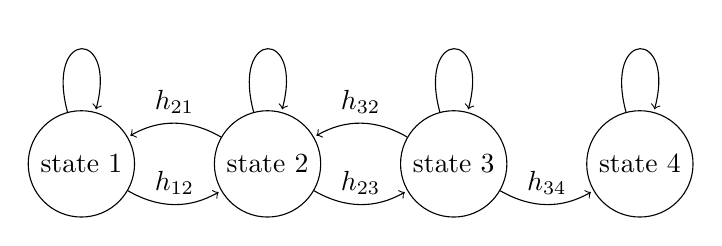
\begin{tikzpicture}
        \node[state]             (1) {state 1};
        \node[state, right=of 1] (2) {state 2};
        \node[state, right=of 2] (3) {state 3};
        \node[state, right=of 3] (4) {state 4};

        \draw[every loop]
            (1) edge[bend right, auto=left]  node {$h_{12}$} (2)
            (2) edge[bend right, auto=right] node {$h_{21}$} (1)
            (2) edge[bend right, auto=left]  node {$h_{23}$} (3)
            (3) edge[bend right, auto=right] node {$h_{32}$} (2)
            (3) edge[bend right, auto=left]  node {$h_{34}$} (4)
            (1) edge[loop above]             node {} (1)
            (2) edge[loop above]             node {} (2)
            (3) edge[loop above]             node {} (3)
            (4) edge[loop above]             node {} (4);
\end{tikzpicture}

\end{document}
